% debut d'un fichier latex standard
\documentclass[a4paper,12pt,twoside]{article}
% Tout ce qui suit le symbole "%" est un commentaire
% Le symbole "\" désigne une commande LaTeX

% pour l'inclusion de figures en eps,pdf,jpg, png
\usepackage{graphicx}

% quelques symboles mathematiques en plus
\usepackage{amsmath}

% le tout en langue francaise
\usepackage[french]{babel}

% on peut ecrire directement les caracteres avec l'accent
%    a utiliser sur Linux/Windows (! dépend de votre éditeur !)
%\usepackage[utf8]{inputenc} % 
%\usepackage[latin1]{inputenc} % Pour Kile
\usepackage[T1]{fontenc}

%    a utiliser sur le Mac ???
%\usepackage[applemac]{inputenc}

% pour l'inclusion de liens dans le document 
\usepackage[colorlinks,bookmarks=false,linkcolor=blue,urlcolor=blue]{hyperref}
\usepackage{wrapfig}
\usepackage{subcaption}
\usepackage{caption}
\usepackage{float}

\paperheight=297mm
\paperwidth=210mm

\setlength{\textheight}{235mm}
\setlength{\topmargin}{-1.2cm} % pour centrer la page verticalement
%\setlength{\footskip}{5mm}
\setlength{\textwidth}{16.5cm}
\setlength{\oddsidemargin}{0.0cm}
\setlength{\evensidemargin}{-0.3cm}

\pagestyle{plain}

% nouvelles commandes LaTeX, utilis\'ees comme abreviations utiles
\def \be {\begin{equation}}
\def \ee {\end{equation}}
\def \dd  {{\rm d}}

\newcommand{\mail}[1]{{\href{mailto:#1}{#1}}}
\newcommand{\ftplink}[1]{{\href{ftp://#1}{#1}}}
%
% latex SqueletteRapport.tex      % compile la source LaTeX
% xdvi SqueletteRapport.dvi &     % visualise le resultat
% dvips -t a4 -o SqueletteRapport.ps SqueletteRapport % produit un PostScript
% ps2pdf SqueletteRapport.ps      % convertit en pdf

% pdflatex SqueletteRapport.pdf    % compile et produit un pdf

% ======= Le document commence ici ================================

\begin{document}

% Le titre, l'auteur et la date
\title{Physique numérique Exercice 1}
\author{Armand Le Douarec, Maxime Chatelin\\  % \\ pour fin de ligne
{\small \mail{armand.ledouarec@epfl.ch}, \mail{maxime.chatelin@epfl.ch}}}
\date{\today}\maketitle
\tableofcontents % Table des matieres

% Quelques options pour les espacements entre lignes, l'indentation 
% des nouveaux paragraphes, et l'espacement entre paragraphes
\baselineskip=16pt
\parindent=0pt
\parskip=12pt

\section{Introduction}

Dans cette étude, nous analysons numériquement le comportement d’une aiguille aimantée soumise à un champ magnétique oscillant. En modélisant le système comme une tige mince pivotant autour de son centre de masse, nous établissons les équations du mouvement et explorons différents régimes dynamiques. Nous nous intéressons notamment aux petits mouvements autour de l’équilibre, à l’excitation paramétrique et aux phénomènes non linéaires tels que le chaos et les attracteurs étranges. Du point de vue numérique, nous implémentons et testons un schéma symplectique, le schéma de Verlet, afin d’évaluer sa stabilité et sa précision, notamment en ce qui concerne la conservation de l’énergie mécanique et l’évolution des trajectoires dans l’espace de phase.

\section{Calculs analytiques}

\subsection{Équation différentielle du mouvement de l'aiguille}

On considère une aiguille aimantée de moment magnétique $\vec{\mu}$, considérée comme une tige mince de masse $m$, de longueur $L$. L'aiguille peut pivoter autour de son centre de masse $G$ dans le plan horizontal $(x, y)$. On note $\vec{w}$ sa vitesse angulaire de rotation, $\vec{w} = w\hat{z}$. Le moment d'inertie de l'aiguille $I_G$ est calculé de la manière suivante :\\

\begin{equation}
    I_G = \int^m_0 r^2\,\text{d}m \quad \Rightarrow \quad I_G = \int^{\frac{L}{2}}_{-\frac{L}{2}} r^2\frac{m}{L}\,\text{d}r \quad \Rightarrow \quad I_G = \displaystyle\frac{1}{12}mL^2
    \label{eq1}
\end{equation}

Ici, on notera $\theta$ l'angle que fait l'aiguille avec l'axe $x$. On a donc $\vec{w}=\dot{\theta}\hat{z}$.
L'aiguille est soumise à un couple de force magnétique $\vec{M}=\vec{\mu}\times\vec{B}$ et un couple de force de viscosité $\vec{M_v}=-\kappa\dot{\theta}\hat{z}$. D'après le théorème du moment cinétique,

\[
\vec{M}+\vec{M_v} = \displaystyle\frac{\text{d}\vec{L}}{\text{d}t} \quad\text{, où } \vec{L} = I_G\vec{w} 
\]
\begin{equation}
\Rightarrow \quad\vec{M}+\vec{M_v} = \displaystyle\frac{\text{d}(I_G\vec{w})}{\text{d}t}=I_G\displaystyle\frac{\text{d}\vec{w}}{\text{d}t}=I_G\dot{\vec{w}}
\label{eq2}
\end{equation}

L'expression du champ magnétique est la suivante :\\
\[
\vec{B}(t)= (B_0+B_1\sin(\Omega t))\,\hat{x}
\]
\noindent avec des amplitudes $B_0$ et $B_1$ données et une fréquence angulaire $\Omega$ donnée.

À partir du champ magnétique $\vec{B}$, on obtient l'expression de $\vec{M} +\vec{M_v}$, donnée par :\\
\begin{equation}
\vec{M}+\vec{M_v} = \vec{\mu}\times(B_0+B_1\sin(\Omega t))\,\hat{x} -\kappa\dot{\theta}\hat{z}
\label{eq3}
\end{equation}

On simplifie l'expression en exprimant le moment magnétique $\vec{\mu}$ à partir des vecteurs unitaires $\hat{x}$ et $\hat{y}$. On a donc : 
\[
\vec{\mu} = \cos(\theta)\hat{x} + \sin(\theta)\hat{y}
\]
On obtient alors l'équation du mouvement à partir des équations Eq.(\ref{eq1}), Eq.(\ref{eq2}) et Eq.(\ref{eq3}):

\begin{equation}
    \mu\sin(\theta)(B_0+B_1\sin(\Omega t)) + \kappa\dot{\theta} = -\displaystyle\frac{1}{12}mL^2\ddot{\theta}
    \label{eq4}
\end{equation}

Soit $\vec{y}$ le vecteur défini par $\vec{y} = (\theta,\dot{\theta})$. Il représente les vecteurs vitesse et position de l'aiguille.
\begin{equation}
\displaystyle\frac{\text{d}\vec{y}}{\text{d}t} = \vec{f}(\vec{y}) = \left(
\begin{tabular}{c}
     $\dot{\theta}$ \\
     $-\displaystyle\frac{12}{mL^2}\left[\mu \sin(\theta)(B_0+B_1\sin(\Omega t)) +\kappa\dot{\theta}\right]$
\end{tabular}
\right)
\end{equation}
\subsection{Énergie mécanique}

Soit $E_{mec}$ l'énergie mécanique de l'aiguille. En effet, l'énergie mécanique de l'aiguille est la somme de son énergie cinétique $E_{cin}$ et son énergie potentielle $E_{pot}$. On obtient donc :\\
\[
E_{cin} = \displaystyle\frac{1}{2}I_Gw^2=\displaystyle\frac{1}{24}mL^2\dot{\theta}^2
\]
\[
E_{pot}=-\vec{\mu}\cdot\vec{B}=-\mu B_0\cos(\theta)
\]
\begin{equation}
  E_{mec} =  E_{cin} +E_{pot} =\displaystyle\frac{1}{24}mL^2\dot{\theta}^2 -\mu B_0\cos(\theta)
\end{equation}

L'énergie mécanique n'est pas conservée car la force de viscosité travaille et l'aiguille est excitée par une force magnétique d'excitation non constante. La somme des puissances des forces non conservatives est donc :\\
\[
P_{mag}=(\vec{\mu}\times\vec{B}_{nc})\cdot{\vec{w}}=-\mu (B_1\sin(\Omega t))\sin(\theta)\hat{z}\cdot\dot{\theta}\hat{z}=-\mu (B_1\sin(\Omega t))\sin(\theta)\dot{\theta}
\]
\[
P_{v}=- \kappa\dot{\theta}\hat{z}\cdot\dot{\theta}\hat{z}=- \kappa\dot{\theta}^2
\]
\begin{equation}
\sum P_{nc} = -\mu B_1\sin(\Omega t)\sin(\theta)\dot{\theta} - \kappa\dot{\theta}^2
\end{equation}

\subsection{Approximation au voisinage de la position d'équilibre $\theta_{eq}=0$ dans le cas sans viscosité et sans excitation}

Dans le cas sans excitation, l'amplitude de l'excitation est nulle, $B_1 = 0$ et sans viscosité, le facteur de viscosité est nul $\kappa = 0$. En effectuant l'approximation autour de la position d'équilibre $\theta_{eq} = 0$, le développement en série de Taylor du sinus à l'ordre 1 donne $\sin(\theta) = \theta + o(\theta)$. On obtient donc, à partir de l'Eq.(\ref{eq4}), l'équation du mouvement suivante :
\begin{equation}
    \ddot{\theta} = -\displaystyle\frac{12B_0\mu}{mL^2}\theta
\end{equation}
On a donc la fréquence propre $\omega_0=\displaystyle\sqrt{\frac{12B_0\mu}{mL^2}}$ et le mode propre suivant :\\

\begin{equation}
    \theta(t) = A\sin(\omega_0t+\phi)
\end{equation}

\noindent où $A$ et $\phi$ sont des constantes que l'on détermine à partir des conditions initiales $\theta(t=0) = \theta_0$ et $\dot{\theta}(t=0) = \dot{\theta}_0$ :\\
Dans le cas où  $\theta_0 = 0$, on a $\phi = 0$ et $A = \frac{\dot{\theta}_0}{\omega_0}$ \\
Dans le cas où $\dot{\theta}_0 = 0$, on a $\phi =\eta \frac{\pi}{2}$ et $A = \eta\theta_0$ avec $\eta = \pm 1$. \\
Si l'on ne se trouve pas dans l'un de ces deux cas, on a :
\begin{equation}
    \left\{ \begin{tabular}{c}
      $A\sin(\phi)=\theta_0$     \\
      $A\omega_0\cos(\phi)=\dot{\theta}_0$ 
    \end{tabular}
    \right.
    \quad\Rightarrow\quad
    \left\{ \begin{tabular}{c}
      $\phi=\displaystyle\arctan\left(-\frac{\theta_0}{\dot{\theta}_0}\right)$     \\
      $A = \displaystyle\sqrt{\theta_0^2 + \left(\frac{\dot{\theta}_0}{\omega_0}\right)^2}$
    \end{tabular}
    \right.
\end{equation}

\subsection{Analyse des forces exercées sur l'aiguille aimantée}

Au point d'équilibre, la somme des couples exercés par le champ magnétique statique et la viscosité est nulle. Cependant, lorsque le champ magnétique oscille, il induit un couple variable qui met l'aiguille en mouvement. Ce couple d'excitation magnétique est responsable de l'accélération initiale de l'aiguille et peut l'éloigner de sa position d'équilibre, rendant ainsi le système potentiellement instable. Lorsque l'aiguille acquiert une vitesse angulaire non nulle, le couple de viscosité entre en jeu. Il est proportionnel à la vitesse angulaire et agit dans le sens opposé, dissipant l'énergie et freinant la rotation. Ce phénomène joue un rôle clé dans la stabilisation ou l’amortissement des oscillations de l’aiguille, influençant la dynamique globale du système.

\section{Implémentation en C++}

L'implémentation des schémas numériques est réalisée en C++. Nous définissons les équations différentielles du mouvement dans un référentiel tournant et utilisons une intégration discrète pour simuler la trajectoire du satellite.

\subsection{Définition des constantes et des structures de données}

Nous définissons d'abord les constantes physiques utilisées dans la première étape de la simulation, ainsi que les structures de données permettant de stocker les informations relatives à l'aiguille.

\begin{verbatim}
// Constantes physiques
Omega = 1.0
kappa = 0
m = 0.075
L = 0.08
B0 = 0.01
mu = 0.2
theta0 = 1e-6
thetadot0 = 0
sampling = 1
N_excit = 0
Nperiod = 3
nsteps = [100,200,500,1000,5000,10000,100000]

\end{verbatim}

\hspace{1cm}

\begin{wrapfigure}{h}{0.5\textwidth}
    \centering
    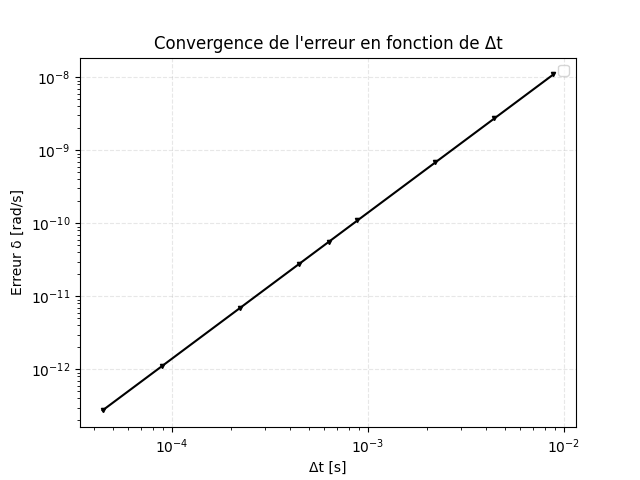
\includegraphics[width=1\linewidth]{graphes/question_1_log.png}
    \captionsetup{justification=centering}
    \caption{Diagramme log-log de l'erreur de $\delta$ en fonction de $\Delta t$.}
    \label{fig1}
\end{wrapfigure}

\subsection{Petits mouvements. Mode propre.}

La première partie de cet exercice considère le cas sans excitation, proche du point d'équilibre stable $\theta_{eq} = 0$ rad avec $\theta_0=10^{-6}$\, rad et $N=3$ périodes. La Fig.(\ref{fig1}) présente un diagramme log-log pour évaluer l'erreur $\delta$ de la position finale par rapport au résultat théorique attendu en fonction des différentes valeurs de $\Delta t$ correspondant au  pas de temps.

\vspace{-0.5cm}
\[
\hspace{-0.3cm}
\delta = \\ \sqrt{\omega^2_0 (\theta(t_{\text{fin}}) - \theta_a(t_{\text{fin}}))^2 + (\dot{\theta}(t_{\text{fin}}) - \dot{\theta}_a(t_{\text{fin}}))^2} \\
\]

\noindent où $\omega_0$ correspond à la fréquence angulaire propre et $\theta_a$ la solution analytique.

\clearpage

La ligne droite de la Fig.(\ref{fig1}) représente la convergence vers la valeur théorique trouvée à partir des calculs analytiques. De plus, la pente de la droite étant de 2, on en déduit que la convergence est d'ordre 2.

\subsection{Excitation paramétrique.} \label{sec3.3}

Dans le cas suivant, on ajoute à l'aiguille une excitation paramétrique. On définit $B_1$ l'amplitude du champ magnétique de l'excitation, $ B_1=0.002$ T et le nombre de périodes d'excitation $N_{excit}=100$. Désormais, $\Omega = 2\omega_0$ et on cherche à observer l'évolution de $\theta$ en fonction du temps ainsi que le portrait de phase, présentés dans les Fig.(\ref{fig2}) et Fig.(\ref{fig3}). De plus, la trace de l'énergie mécanique et la comparaison de la dérivée temporelle de l'énergie mécanique et de la puissance des forces non conservatives sont montrées Fig(\ref{fig4}) et Fig.(\ref{fig5}).

\begin{figure}[H]
    \centering
    \begin{minipage}{0.47\textwidth}
        \centering
        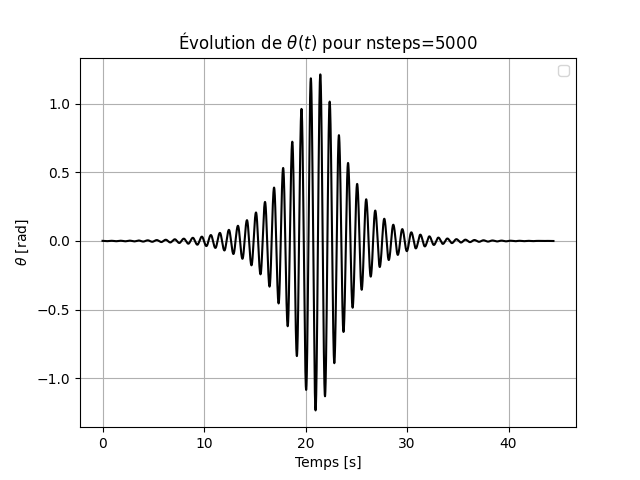
\includegraphics[width=\linewidth]{graphes/question_2_theta_t.png}
        \captionsetup{justification=centering}
        \caption{Variation de l'angle $\theta$ en fonction du temps.}
        \label{fig2}
    \end{minipage}
    \hfill
    \begin{minipage}{0.47\textwidth}
        \centering
        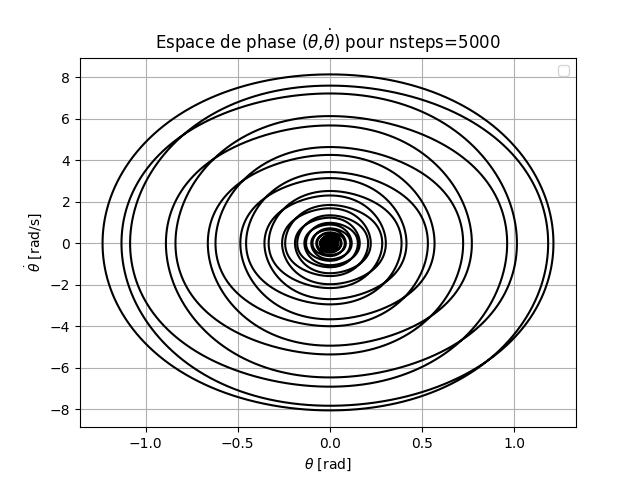
\includegraphics[width=\linewidth]{graphes/question_2_portrait_phase.png}
        \captionsetup{justification=centering}
        \caption{Portrait de phase de l'aiguille aimantée.}
        \label{fig3}
    \end{minipage}
\end{figure}

\begin{figure}[H]
    \centering
    \begin{minipage}{0.47\textwidth}
        \centering
        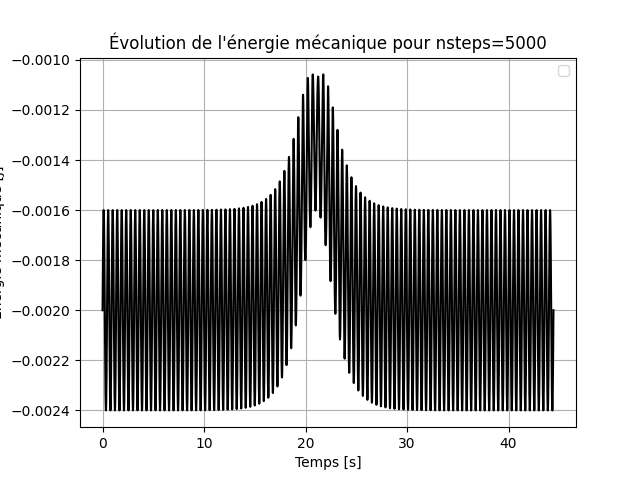
\includegraphics[width=\linewidth]{graphes/question_2_E_mec_manquant.png}
        \captionsetup{justification=centering}
        \caption{Trace temporelle de $E_{mec}$.}
        \label{fig4}
    \end{minipage}
    \hfill
    \begin{minipage}{0.47\textwidth}
        \centering
        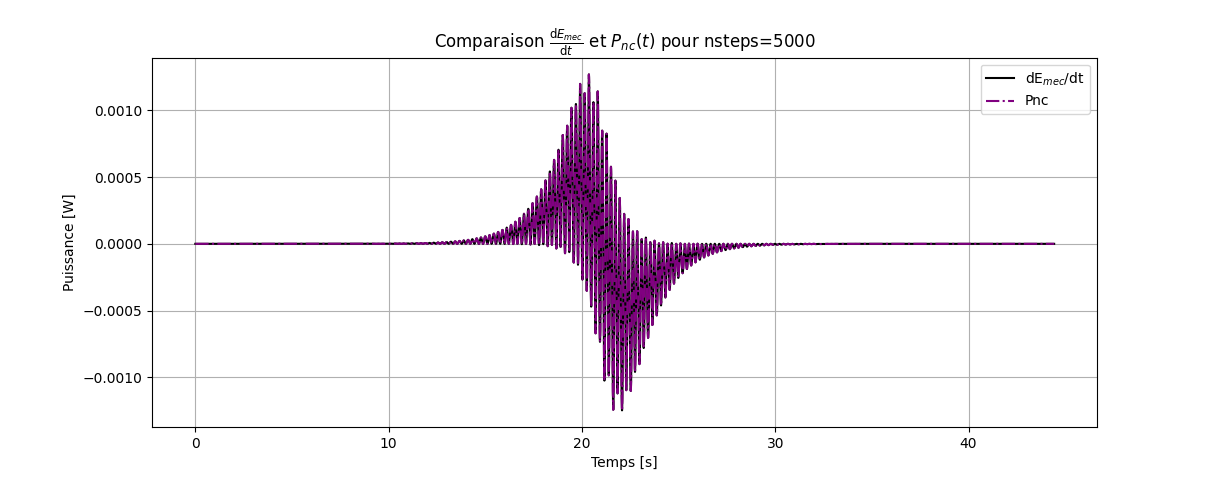
\includegraphics[width=\linewidth]{graphes/question_2_E_mec.png}
        \captionsetup{justification=centering}
        \caption{Comparaison de $dE_{mec}/dt$ et $P_{nc}$ au cours du temps.}
        \label{fig5}
    \end{minipage}
\end{figure}

Le choix $\Omega = 2 \cdot \omega_0$ induit une résonance paramétrique, permettant un transfert d’énergie efficace vers l’oscillation de l’aiguille. Cette perturbation a lieu aux alentours de $t=20$\,s. Cela entraîne une augmentation de l’énergie mécanique puis un retour à l'état initial et un changement dans $P_{nc}$ ou $dE_{mec}/dt$, qui sont égales, ce qui est en accord avec la théorie. L'élargissement des orbites du portrait de phase illustre l’injection régulière d’énergie par l’excitation paramétrique. Mais $B_1$ étant assez faible, le système ne devient pas chaotique, reste borné comme l'indique le portrait de phase. L'élargissement des orbites du portrait de phase illustre l’induction régulière d’énergie par l’excitation paramétrique. Le portrait de phase montre que l’aiguille part de son point d’équilibre (0,\,0), puis s’en écarte sous l’effet de l’excitation, traçant des orbites elliptiques caractéristiques d’un mouvement sinusoïdal de l’angle $\theta$. Enfin, après excitation, la particule converge de nouveau vers son point d’équilibre.


\vspace{-0.5cm}

\subsection{Sections de Poincaré. Cas sans amortissement.}  \label{sec3.4}

\vspace{-0.3cm}

Les sections de Poincaré sont analysés à partir des mêmes paramètres que la section précédente sauf pour le nombre de période d'excitation $N_{excit}=10000$ et du nombre de pas de temps par excitation $n_{steps}=10$. La position et la vitesse de l'angle $\theta$ sont relevées à chaque période. Les différentes couleurs dans la Fig.(\ref{fig6}) des sections de Poincaré correspondent aux différentes conditions initiales.

\vspace{-0.3cm}

\begin{figure}[H]
    \centering
    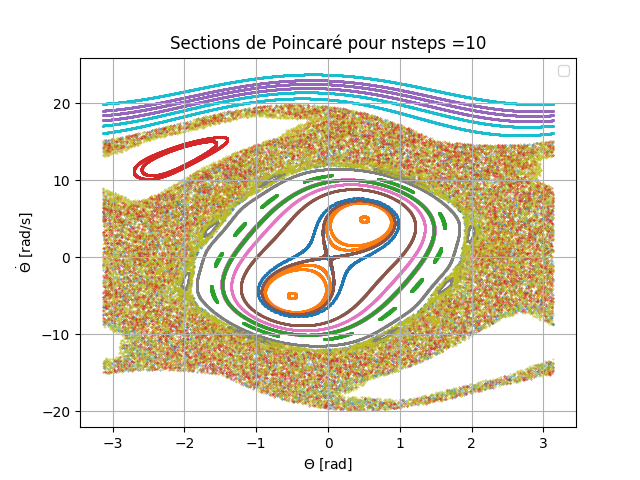
\includegraphics[width=0.7\textwidth]{graphes/question_3.png}
    \captionsetup{justification=centering}
    \caption{Sections de Poincaré de l'aiguille aimantée sans amortissement.}
    \label{fig6}
\end{figure}

\vspace{-0.4cm}

Trois solutions sont observables sur la Fig.(\ref{fig6}). Il s'agit du portrait de phase de l'aiguille. Par conséquent, chaque cas présente une orbite différente dans le portrait de phase. Le premier type qui se distingue est le mouvement borné et non chaotique proche des positions d'équilibre de l'aiguille et à faible vitesse comme pour la courbe orange, verte ou rouge. L'énergie mécanique étant conservée, le volume de ces orbites reste constant, ce sont des orbites fermées représentant des oscillations harmoniques. D'autres mouvements non bornée mais prédictible sont observables présentés ici par les courbe turquoises et violettes pour des vitesses très élevées. L'amplitude de la perturbation est insuffisante pour rendre le mouvement de l'aiguille chaotique et l'orbite est donc ouverte. Enfin, l'apparition du chaos s'observe avec des points qui semblent apparaître à des endroits aléatoires entre les orbites stables autour de la position d'équilibre et les orbites. Ceci est bien montré par le nuage de points de teint jaunâtre.

\vspace{-0.4cm}

\subsection{Chaos, stabilité des orbites (Lyapunov). Cas sans amortissement.}

\vspace{-0.2cm}

Cette partie reprend les mêmes paramètres que les deux questions précédentes et vise à étudier deux simulations "quasi-jumelles", obtenues avec des angles initiaux qui diffèrent de $10^{-6}$\,rad. L'étude de la stabilité des orbites de l'aiguille se font dans le cas de comportements chaotique et non-chaotique. Pour décrire la stabilité des orbites, la "distance" (qui en réalité n'en est pas véritablement une) $\delta_{ab}(t)$ entre les deux orbites de l'aiguille à chaque pas de temps est analysée. Elle est définie par :



\[
\delta_{ab}(t) = \sqrt{\omega^2_0 (\theta_b(t) - \theta_a(t))^2 + (\dot{\theta}_b(t) - \dot{\theta}_a(t))^2}
\]



\noindent où $\theta_a(t)$ et $\theta_b(t)$ sont les positions de chaque simulation. La Fig.(\ref{fig7a}) présente les deux cas possibles quant à la Fig.(\ref{fig7b}), il s'agit d'un zoom sur le cas non chaotique. 

\begin{figure}[H]
\begin{subfigure}{0.5\textwidth}  % Réduire la taille pour s'assurer qu'elles tiennent côte à côte
    \centering  % Centrer cette sous-figure
    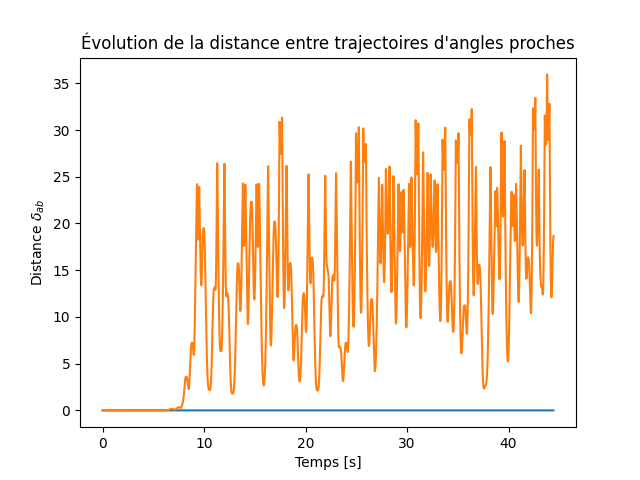
\includegraphics[scale=0.5]{graphes/question_4.png}
    \caption{}
    \label{fig7a}
\end{subfigure}
\hspace{0.01\textwidth}
\begin{subfigure}{0.5\textwidth}  % Réduire également ici
    \centering  % Centrer cette sous-figure
    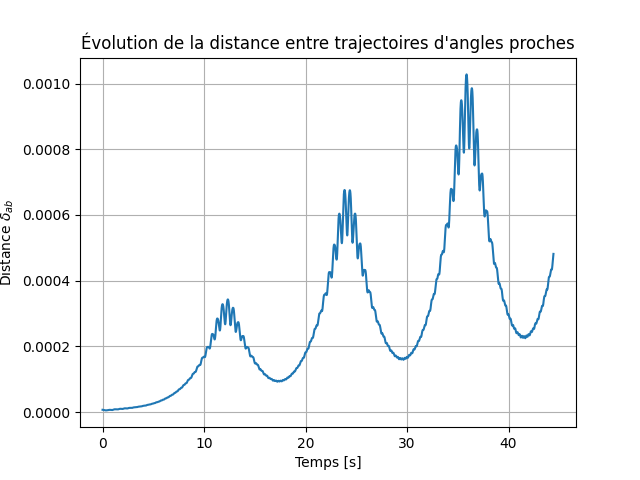
\includegraphics[scale=0.5]{graphes/question_4_zoom.png}
    \caption{}
    \label{fig7b}
\end{subfigure}
\captionsetup{justification=centering}
\caption{Distance $\delta _{ab}$ en fonction du temps pour les cas (a) non-chaotique ($\theta_0=1$\,rad et $\dot{\theta}=5$\,rad/s) et chaotique ($\theta_0=1$\,rad et $\dot{\theta}=15$\,rad/s), avec (b) un zoom sur le cas non-chaotique.}

\label{fig7}
\end{figure}


Dans le cas non chaotique, la distance entre les deux situations "quasi-jumelles" est très faible par rapport au cas chaotique. En effet, dans un cas stable, à partir de la position de l'aiguille connue d'une des deux simulations, il est possible d'approximer correctement la position de l'aiguille dans l'autre simulation. Le zoom sur le cas non chaotique montre que $\delta _{ab}(t)$ suit bien un comportement solution de l'équation différentielle. Elle est la somme d'une composante linéaire d'ordre 1 $\alpha\,t$ et d'une somme de sinusoïdales ayant différentes fréquences. Ici, c'est la valeur absolue des sinusoïdales qui a été implémentée. Dans le cas chaotique, un terme exponentiel $e^{\lambda t}$, avec le coefficient chaotique $\lambda$ de Lyapunov, s'ajoute pour décrire le comportement de la distance $\delta _{ab}(t)$. Le coefficient de Lyapunov mesure la sensibilité aux conditions initiales. Sa positivité est une caractéristique du mouvement chaotique et décrit ainsi une divergence exponentielle.Par conséquent, $\delta _{ab}(t)$ diverge de manière exponentielle  avant d'osciller fortement autour d'une valeur limite représentant sa valeur de saturation. Cette saturation est une conséquence de l'énergie du système qui n'est pas infinie, la distance $\delta _{ab}(t)$ est ainsi bornée, c'est la borne énergétique du système. Cependant, malgré la valeur de saturation, le mouvement de la deuxième simulation est imprédictible à partir des données de la première après la divergence exponentielle de $\delta _{ab}(t)$ car l'amplitude oscillation et sa pulsation sont de l'ordre respectivement de dizaines de radians et de plusieurs radians par seconde. Malgré la faible différence des conditions initiales, la divergence des comportements de l'aiguille se constate rapidement, dès la dixième seconde de la simulation qui représente ici la limite de prédictibilité. À partir des positions d'une des deux simulations, trouver une approximation de la position de l'autre simulation n'est pas possible.

\subsection{Chaos, attracteurs étranges. Cas avec amortissement}

On reprend maintenant simplement la situation de la partie (\ref{sec3.4}) mais avec une constante d'amortissement $\kappa$ non nulle. Les valeurs des paramètres sont alors $\kappa=2\cdot10^{-5}$ et $B_1=0.018$\,T. Alors la Fig.(\ref{fig8}) nous présente les sections de Poincaré dans deux cas avec pour condition initiale $\theta=-1$\,rad, $\dot{\theta}=-8$\,rad/s et $\theta=-2$\,rad, $\dot{\theta}=50$\,rad/s.

La section de Poincaré, visible sur la Fig.(\ref{fig8a}),admet une certaine symétrie centrale autour du point $(0,0)$. Cette caractéristique suggère la conservation de certaines propriétés dynamiques. Le mouvement n'est ni périodique, ni aléatoire mais présente une structure fractale, la forme atypique obtenue ici en témoigne. On parle d'attracteur étrange, toutes les trajectoires, malgré des conditions initiales tout à fait différentes convergent vers ce même attracteur. La même simulation, pour les paramètres $\theta=-2$\,rad et $\dot{\theta}=50$\,rad/s , est visible sur la Fig.(\ref{fig8b}). On observe bien que la trajectoire converge vers le même attracteur étrange. L’introduction d’un amortissement change radicalement la dynamique. Au lieu d’une divergence exponentielle comme dans le cas purement chaotique, les trajectoires convergent vers une structure complexe appelée attracteur étrange. L'existence de cet attracteur ne garantit pas une prédictibilité du système mais permet d'interdire toute évolution divergente, complètement aléatoire, de la trajectoire.


\begin{figure}[H]
\begin{subfigure}{0.5\textwidth}  % Réduire la taille pour s'assurer qu'elles tiennent côte à côte
    \centering  % Centrer cette sous-figure
    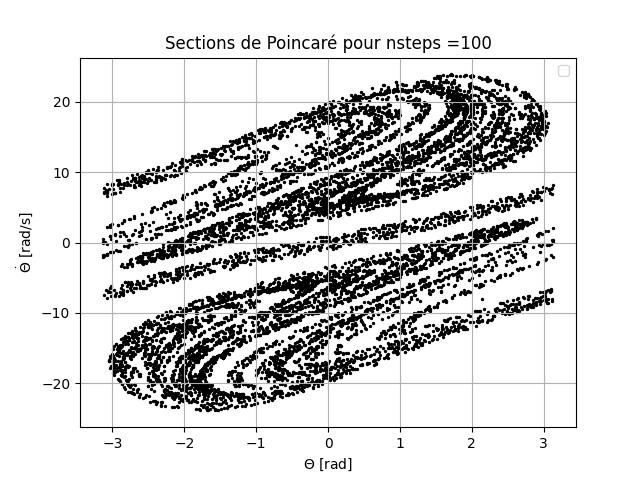
\includegraphics[scale=0.5]{graphes/question_5_b.png}
    \caption{}
    \label{fig8a}
\end{subfigure}
\hspace{0.01\textwidth}
\begin{subfigure}{0.5\textwidth}  % Réduire également ici
    \centering  % Centrer cette sous-figure
    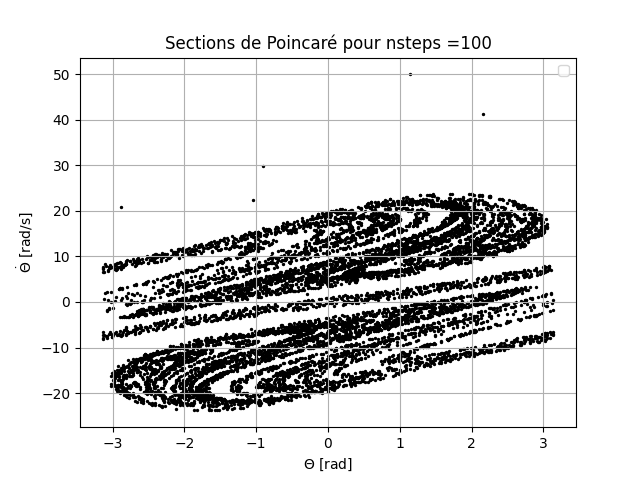
\includegraphics[scale=0.5]{graphes/question_5_attracteur.png}
    \caption{}
    \label{fig8b}
\end{subfigure}
\captionsetup{justification=centering}
\caption{Sections de Poincaré de l'aiguille aimantée avec amortissement pour (a) $\theta=-1$\,rad et $\dot{\theta}=-8$\,rad/s et (b) $\theta=-2$\,rad et $\dot{\theta}=50$\,rad/s.}
\label{fig8}
\end{figure}


\subsection{Facultatif}

Dans cette partie, on reprend les paramètres de la section (\ref{sec3.3}) et comme condition initiale $\theta=\pi$, $\dot{\theta}=0$ d'abord essayé de stabiliser dans le cas chaotique l'angle de l'aiguille autour de $\theta_{eq}=\pi$, un point d'équilibre instable. Pour ce faire, plusieurs sources de stabilisation ont été testées. Dans l'accélération du code python, on a rajouté deux composantes : $C(\theta - \pi)$ qui est un gain de rappel qui pousse $\theta$ vers $\pi$, ainsi que $\alpha \cos(\beta t + \gamma)$, une force périodique ayant pour but de compenser les oscillations autour de la solution désirée. 

\begin{figure}[H]
\centering
\begin{subfigure}{0.45\textwidth}  % Réduire la taille pour s'assurer qu'elles tiennent côte à côte
    \centering  % Centrer cette sous-figure
    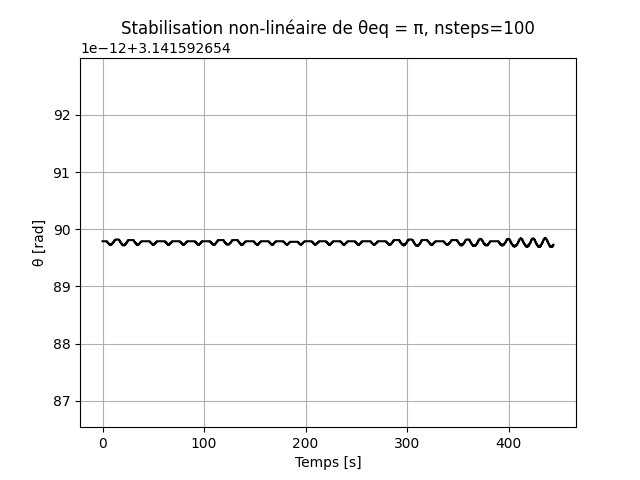
\includegraphics[scale=0.52]{graphes/facultatif_nsteps_100.png}
    \caption{}
    \label{fig9a}
\end{subfigure}
\hspace{0.05\textwidth}
\begin{subfigure}{0.45\textwidth}  % Réduire également ici
    \centering  % Centrer cette sous-figure
    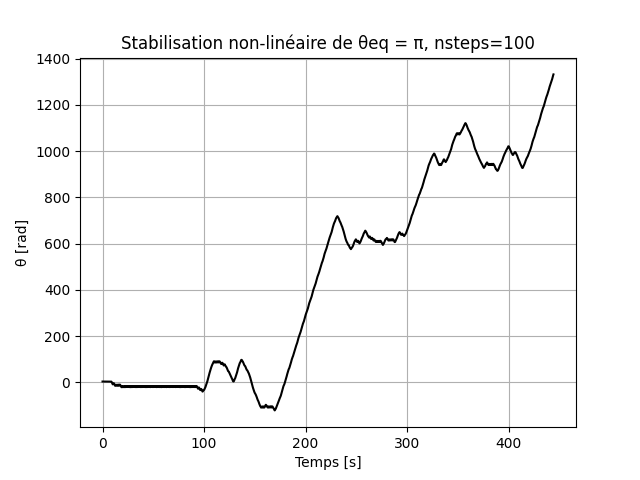
\includegraphics[scale=0.52]{graphes/facultatif_C_0.png}
    \caption{}
    \label{fig9b}
\end{subfigure}
\captionsetup{justification=centering}
\caption{Graphe de $\theta(t)$ avec $\theta_0=\pi$ pour (a) $C=50$ comme unique force stabilisatrice et (b) $C=0$ donc sans force de rappel.}
\label{fig9}
\end{figure}

Après différentes expériences, le meilleur stabilisateur s'avère être la force de rappel avec une constante $C$ suffisamment élevée. Par exemple, pour une condition initiale à $\pi$, la Fig.(\ref{fig9a}) montre ce qui se passerait pour $C=50$ et affiche un angle $\theta$ proche de $\pi$ avec une précision de $10^{-12}$ environ, et ce peu importe la durée de la simulation ! La Fig.(\ref{fig9b}) montre alors ce qu'il se passerait sans constante de rappel,  $C=0$.




\section{Conclusion}

Dans cette étude, nous avons analysé le comportement dynamique d’une aiguille aimantée soumise à un champ magnétique oscillant en combinant modélisation mathématique et simulations numériques en C++. Nos résultats ont révélé une grande diversité de régimes dynamiques, allant d’un alignement stationnaire aux oscillations périodiques, jusqu’à des comportements plus complexes comme l’excitation paramétrique et le chaos, mis en évidence par les sections de Poincaré et les exposants de Lyapunov. Ces phénomènes illustrent la richesse des systèmes non linéaires et trouvent des analogies avec des modèles classiques comme le pendule paramétrique ou le système de Duffing. Au-delà du cas spécifique étudié, ce travail met en lumière les subtilités des interactions entre excitation externe et réponse dynamique, soulignant l’importance des méthodes numériques et analytiques pour appréhender ces phénomènes et ouvrant la voie à de nouvelles investigations en physique fondamentale et appliquée.

\end{document} %%%% THE END %%%%
